\documentclass{article}
\usepackage[T1]{fontenc}
\usepackage[preprint]{colm2026_conference}

\usepackage{microtype}
\usepackage{hyperref}
\usepackage{url}
\usepackage{xurl}
\usepackage{booktabs}
\usepackage{graphicx}
\usepackage{amsmath,amssymb}
\usepackage{xcolor}
\usepackage{listings}
\usepackage{algorithm}
\usepackage{algpseudocode}
\definecolor{citeblue}{rgb}{0.16, 0.42, 0.73}
\hypersetup{colorlinks=true, citecolor=citeblue, linkcolor=citeblue, urlcolor=citeblue}
\usepackage[capitalize,noabbrev]{cleveref}
\lstset{basicstyle=\ttfamily\footnotesize, breaklines=true, breakatwhitespace=true, columns=fullflexible, frame=single, framerule=0.3pt, rulecolor=\color{gray!60}, xleftmargin=4pt, xrightmargin=4pt, aboveskip=6pt, belowskip=8pt}

% Scores from the original evaluation (November 2025). Transcribed from the scoring records; see Section 4 for how they were produced.
% Automated debate evaluation, three topics, both sides, six transcripts.
\newcommand{\autoStanceDC}{91}\newcommand{\autoStanceOAI}{68}
\newcommand{\autoCoherenceDC}{8.8}\newcommand{\autoCoherenceOAI}{7.2}
\newcommand{\autoEvidenceDC}{8.9}\newcommand{\autoEvidenceOAI}{7.1}
\newcommand{\autoRebuttalDC}{8.7}\newcommand{\autoRebuttalOAI}{7.0}
\newcommand{\autoPersuasionDC}{8.5}\newcommand{\autoPersuasionOAI}{7.6}
\newcommand{\autoFluencyDC}{7.7}\newcommand{\autoFluencyOAI}{8.6}
% Human-coded evaluation, ten prompts, one blind rater.
\newcommand{\humSupportedDC}{0.80}\newcommand{\humSupportedOAI}{0.68}\newcommand{\humSupportedStorm}{0.60}
\newcommand{\humUtilDC}{0.76}\newcommand{\humUtilOAI}{0.67}\newcommand{\humUtilStorm}{0.61}
\newcommand{\humLogicDC}{7.7}\newcommand{\humLogicOAI}{6.5}\newcommand{\humLogicStorm}{6.0}
\newcommand{\humStanceDC}{9}\newcommand{\humStanceOAI}{1}\newcommand{\humStanceStorm}{2}

% Generated by scripts/text_analysis.py. Do not edit by hand.
\newcommand{\bibMaxDc}{39}
\newcommand{\bibMedDc}{36}
\newcommand{\bibMinDc}{30}
\newcommand{\dagLeafSources}{26}
\newcommand{\dagLeafSourcesMean}{4.3}
\newcommand{\dagLeaves}{6}
\newcommand{\dagMaxDepth}{3}
\newcommand{\dagNodes}{10}
\newcommand{\dagParents}{4}
\newcommand{\dagRefinedNodes}{3}
\newcommand{\dagReportCitations}{213}
\newcommand{\dagReportSources}{26}
\newcommand{\dagReportWords}{3154}
\newcommand{\dagRootAnswerWords}{454}
\newcommand{\dagRootFromRefinement}{9}
\newcommand{\dagRootSources}{26}
\newcommand{\labEndingCompromise}{1}
\newcommand{\labEndingConditional}{2}
\newcommand{\labEndingFirm}{5}
\newcommand{\labEndingQualified}{2}
\newcommand{\labSideAgainst}{1}
\newcommand{\labSideFor}{8}
\newcommand{\labSideNeither}{1}
\newcommand{\labTitleClaim}{9}
\newcommand{\labTitleTopic}{1}
\newcommand{\linkBlocked}{93}
\newcommand{\linkBlockedPct}{27}
\newcommand{\linkChecked}{349}
\newcommand{\linkDead}{15}
\newcommand{\linkDeadPct}{4}
\newcommand{\linkOk}{241}
\newcommand{\linkOkPct}{69}
\newcommand{\nPrompts}{10}
\newcommand{\nReports}{20}
\newcommand{\srcN}{349}
\newcommand{\srcShareAcademic}{21}
\newcommand{\srcShareCompanyBlogOrOther}{42}
\newcommand{\srcShareEncyclopedia}{1}
\newcommand{\srcShareGovernment}{13}
\newcommand{\srcShareNewsOrMagazine}{1}
\newcommand{\srcShareThinkTankOr}{22}
\newcommand{\srcUnique}{346}
\newcommand{\txCausalDc}{4.2}
\newcommand{\txCausalDiff}{+0.3}
\newcommand{\txCausalHi}{+1.8}
\newcommand{\txCausalLo}{-0.5}
\newcommand{\txCausalP}{0.432}
\newcommand{\txCausalSt}{3.0}
\newcommand{\txCausalWins}{5}
\newcommand{\txCiteDensityDc}{5.7}
\newcommand{\txCiteDensityDiff}{+1.0}
\newcommand{\txCiteDensityHi}{+2.1}
\newcommand{\txCiteDensityLo}{+0.0}
\newcommand{\txCiteDensityP}{0.037}
\newcommand{\txCiteDensitySt}{4.7}
\newcommand{\txCiteDensityWins}{8}
\newcommand{\txCitedShareDc}{0.46}
\newcommand{\txCitedShareDiff}{-0.15}
\newcommand{\txCitedShareHi}{-0.09}
\newcommand{\txCitedShareLo}{-0.23}
\newcommand{\txCitedShareP}{0.002}
\newcommand{\txCitedShareSt}{0.60}
\newcommand{\txCitedShareWins}{0}
\newcommand{\txCitesPerSourceDc}{9.3}
\newcommand{\txCitesPerSourceDiff}{+5.0}
\newcommand{\txCitesPerSourceHi}{+7.2}
\newcommand{\txCitesPerSourceLo}{+1.7}
\newcommand{\txCitesPerSourceP}{0.002}
\newcommand{\txCitesPerSourceSt}{4.1}
\newcommand{\txCitesPerSourceWins}{10}
\newcommand{\txCommitDc}{6.8}
\newcommand{\txCommitDiff}{+3.3}
\newcommand{\txCommitHi}{+4.2}
\newcommand{\txCommitLo}{+0.4}
\newcommand{\txCommitP}{0.002}
\newcommand{\txCommitSt}{3.8}
\newcommand{\txCommitWins}{10}
\newcommand{\txContrastDc}{5.5}
\newcommand{\txContrastDiff}{-0.3}
\newcommand{\txContrastHi}{+1.0}
\newcommand{\txContrastLo}{-0.8}
\newcommand{\txContrastP}{0.922}
\newcommand{\txContrastSt}{6.0}
\newcommand{\txContrastWins}{4}
\newcommand{\txHedgeDc}{2.8}
\newcommand{\txHedgeDiff}{-2.2}
\newcommand{\txHedgeHi}{-0.4}
\newcommand{\txHedgeLo}{-7.3}
\newcommand{\txHedgeP}{0.020}
\newcommand{\txHedgeSt}{6.4}
\newcommand{\txHedgeWins}{1}
\newcommand{\txSourcesDc}{8}
\newcommand{\txSourcesDiff}{-18}
\newcommand{\txSourcesHi}{-14}
\newcommand{\txSourcesLo}{-24}
\newcommand{\txSourcesP}{0.002}
\newcommand{\txSourcesSt}{27}
\newcommand{\txSourcesWins}{0}
\newcommand{\txWordsDc}{1339}
\newcommand{\txWordsDiff}{-1172}
\newcommand{\txWordsHi}{-617}
\newcommand{\txWordsLo}{-1621}
\newcommand{\txWordsP}{0.002}
\newcommand{\txWordsSt}{2426}
\newcommand{\txWordsWins}{0}

% Generated by scripts/attribution.py. Do not edit by hand.
\newcommand{\atBibMed}{36}
\newcommand{\atEvalBestChance}{0.10}
\newcommand{\atEvalBestCited}{0.14}
\newcommand{\atEvalCitedBestChance}{0.36}
\newcommand{\atEvalCitedBestCited}{0.41}
\newcommand{\atEvalCitedClaims}{235}
\newcommand{\atEvalCitedMeanCandidates}{6}
\newcommand{\atEvalCitedMedianPct}{0.43}
\newcommand{\atEvalCitedPairs}{491}
\newcommand{\atEvalCitedPctHi}{0.50}
\newcommand{\atEvalCitedPctLo}{0.40}
\newcommand{\atEvalCitedTopThree}{0.56}
\newcommand{\atEvalCitedTopThreeChance}{0.51}
\newcommand{\atEvalClaims}{235}
\newcommand{\atEvalMeanCandidates}{22}
\newcommand{\atEvalMedianPct}{0.47}
\newcommand{\atEvalPairs}{491}
\newcommand{\atEvalPctHi}{0.53}
\newcommand{\atEvalPctLo}{0.40}
\newcommand{\atEvalTopThree}{0.18}
\newcommand{\atEvalTopThreeChance}{0.14}
\newcommand{\atFirstFiveShare}{86}
\newcommand{\atFixBestChance}{0.10}
\newcommand{\atFixBestCited}{0.96}
\newcommand{\atFixClaims}{25}
\newcommand{\atFixMeanCandidates}{26}
\newcommand{\atFixMedianPct}{0.04}
\newcommand{\atFixPairs}{63}
\newcommand{\atFixPctHi}{0.08}
\newcommand{\atFixPctLo}{0.00}
\newcommand{\atFixTopThree}{0.83}
\newcommand{\atFixTopThreeChance}{0.12}
\newcommand{\atLogBestChance}{0.10}
\newcommand{\atLogBestCited}{0.04}
\newcommand{\atLogClaims}{70}
\newcommand{\atLogMeanCandidates}{26}
\newcommand{\atLogMedianPct}{0.48}
\newcommand{\atLogPairs}{173}
\newcommand{\atLogPctHi}{0.52}
\newcommand{\atLogPctLo}{0.44}
\newcommand{\atLogTopThree}{0.06}
\newcommand{\atLogTopThreeChance}{0.12}
\newcommand{\atOldBestChance}{0.10}
\newcommand{\atOldBestCited}{0.52}
\newcommand{\atOldClaims}{25}
\newcommand{\atOldMeanCandidates}{26}
\newcommand{\atOldMedianPct}{0.12}
\newcommand{\atOldPairs}{63}
\newcommand{\atOldPctHi}{0.16}
\newcommand{\atOldPctLo}{0.08}
\newcommand{\atOldTopThree}{0.49}
\newcommand{\atOldTopThreeChance}{0.12}
\newcommand{\atUsedMax}{13}
\newcommand{\atUsedMed}{8}
\newcommand{\atUsedMin}{7}
\newcommand{\atUsedShare}{25}
\newcommand{\atValBestChance}{0.10}
\newcommand{\atValBestCited}{0.96}
\newcommand{\atValClaims}{25}
\newcommand{\atValMeanCandidates}{26}
\newcommand{\atValMedianPct}{0.04}
\newcommand{\atValPagesBestChance}{0.13}
\newcommand{\atValPagesBestCited}{0.84}
\newcommand{\atValPagesClaims}{19}
\newcommand{\atValPagesMeanCandidates}{10}
\newcommand{\atValPagesMedianPct}{0.00}
\newcommand{\atValPagesPairs}{24}
\newcommand{\atValPagesPctHi}{0.11}
\newcommand{\atValPagesPctLo}{0.00}
\newcommand{\atValPagesTopThree}{0.88}
\newcommand{\atValPagesTopThreeChance}{0.30}
\newcommand{\atValPairs}{63}
\newcommand{\atValPctHi}{0.08}
\newcommand{\atValPctLo}{0.00}
\newcommand{\atValTopThree}{0.83}
\newcommand{\atValTopThreeChance}{0.12}

\newcommand{\sys}{De(ep)Composition}

\title{\sys{}: Deep Research for Argumentation\\by Query Decomposition\thanks{Code and data: \url{https://github.com/jessiedong01/deep-research-for-argumentation}}}

\author{Justin Blumencranz \quad Jessie Dong \quad Yucheng Jiang \quad Monica S. Lam \\
Stanford University \\
\texttt{\{jmb25, jessiedong, yuchengj, lam\}@stanford.edu}
}

\begin{document}
\maketitle
\lhead{}
\renewcommand{\footrulewidth}{1.5pt}

\begin{abstract}
Deep research systems search the web and write a cited report, but they are built to summarize. Debate and policy analysis need a position, claims that support it, and evidence for each claim. \sys{} is a deep research pipeline for argumentation. It decomposes a motion into a directed acyclic graph of sub-questions, answers the leaves by web search, composes each parent from its children under generated composition instructions, adds sub-trees where a composed answer is incomplete, and writes a report that argues the root answer. Against OpenAI Deep Research and STORM on ten debate motions, one blind rater scored \sys{}'s reports highest on supported-claims rate, evidence use, and logical connection, and found a firm stance in \humStanceDC{} of 10 reports against \humStanceOAI{} and \humStanceStorm{}; in six automated debates it led on every measure but fluency. Paired measurements on the retained reports confirm the stance difference: compared with STORM, \sys{} uses fewer hedges on nine of ten motions and more commitment markers on all ten, although its conclusions are often softer than its titles. They also show that it cites densely but from few sources, a median of \txSourcesDc{} of the \bibMedDc{} it retrieves. A lexical attribution test, validated on citations known to be correct, finds that the citations in the evaluated reports match their claims no better than chance. The cause is in the pipeline: leaf citation numbers are read against a parent's merged source list, and composition prompts ask for node identifiers instead of sources. The released code fixes both and includes the test as an audit. The rater's supported-claims rate therefore measures how consistently citations are attached, not whether they are correct.

\end{abstract}

\section{Introduction}
\label{sec:intro}

An argumentation task asks for a position and a case for it. A debater, a policy analyst, or an advocate must take a stance, make claims that support it, back each claim with evidence, and answer the other side. Deep research pipelines such as OpenAI Deep Research \citep{openai2025deepresearch} and STORM \citep{shao2024storm} search the web, read what they find, and write a cited report, but their objective is a summary. Asked whether the Federal Reserve should keep interest rates high, they describe both views and stop. For a survey that is the right behavior. For a debate it is a non-answer.

The two kinds of task differ in how research should be organized. A summary can grow bottom-up: search, read, search again where the text is thin, and write up what was found. An argument has a shape before the research starts. The root claim rests on a few supporting claims, each of which rests on evidence, and the research has to fill that structure. This is decomposition, the central move of computational thinking, applied to the logic of an argument instead of the structure of a program: a large question is split into parts that can be answered on their own and then recombined.

\sys{} is a deep research pipeline built on that idea. It first plans: a language model, given the motion and a short literature search, generates a directed acyclic graph (DAG) of sub-questions, in which every non-leaf node also carries instructions for composing its answer from its children. It then researches: leaves are answered by web search, parents are composed from their children in topological order, and a parent whose composed answer is incomplete spawns a sub-tree to fill it. It finally writes: the answered DAG becomes an outline and then a report that argues the root answer. \Cref{fig:pipeline} shows the three phases.

The pipeline was compared with OpenAI Deep Research and STORM in two original evaluations, six automated debates and ten reports scored blind by one rater, in which it scored highest on argument quality and was far more decisive. A second look at the retained reports, which needs no rater, refines both results. Paired lexical measurements confirm that \sys{} commits where STORM hedges, but show that its conclusions are often softer than its titles and that it cites densely from few sources. A citation attribution test then finds a problem the original rubric could not see: the citations in the evaluated reports do not match their claims better than chance. The cause is a provenance failure in recursive composition, in which citation numbers lose their meaning as answers move up the graph, and it can be traced to two lines of the pipeline's design.

\Cref{sec:problem} defines the task and the property of provenance that the pipeline must preserve, \Cref{sec:method} describes the pipeline, \Cref{sec:experiments,sec:results} give the original evaluation with its limits, \Cref{sec:analysis} analyzes what the reports contain, \Cref{sec:citations} presents the attribution test, the diagnosis, and the fix, and \Cref{sec:discussion} states what the results do and do not support. The diagnosis applies to any system that composes cited answers recursively.

\section{Related Work}
\label{sec:related}

\paragraph{Deep research systems.}
OpenAI Deep Research \citep{openai2025deepresearch} is an end-to-end agent that plans searches, browses, and writes a cited report. It was trained with reinforcement learning on browsing tasks of the kind collected in BrowseComp \citep{wei2025browsecomp}, where answers are short facts that are hard to find, so its reward favors retrieval and citation accuracy over the structure of an argument. Its reasoning lives in one context window with no persistent dependency structure between sub-questions. STORM \citep{shao2024storm} writes Wikipedia-like articles: it discovers perspectives on a topic, simulates conversations in which writers with those perspectives question a search-grounded expert, curates the answers into an outline, and writes the article. The questions emerge from the conversations as the research proceeds, so the process is bottom-up, and the output is deliberately balanced. Both systems were designed for summary, and the evaluation below treats them as the strongest available summary-style baselines, not as argumentation systems.

\paragraph{Decomposition and structured reasoning.}
Breaking a problem into sub-problems before solving it is an established prompting strategy: least-to-most prompting \citep{zhou2023leasttomost}, decomposed prompting \citep{khot2023decomposed}, and self-ask \citep{press2023selfask} all have a model generate sub-questions whose answers feed the original question. Tree of Thoughts \citep{yao2023tot} searches over intermediate reasoning steps, ReAct \citep{yao2023react} interleaves reasoning with tool calls, and Graph of Thoughts \citep{besta2024got} generalizes the tree to a graph whose thoughts can merge. These methods target problems with checkable answers, mostly arithmetic, puzzles, or short-form QA. They do not synthesize prose from retrieved evidence, and they do not refine the reasoning structure when a composed answer turns out to be incomplete. \sys{} borrows the decomposition idea and adds composition instructions, evidence-grounded leaves, and gap-driven refinement of the graph.

\paragraph{Multi-agent frameworks.}
AutoGen \citep{wu2023autogen}, CAMEL \citep{li2023camel}, and natural-language societies of mind \citep{zhuge2023mindstorms} coordinate several language-model agents through conversation, with roles such as planner, researcher, and critic. Their communication is flat: agents exchange messages, and the structure of the task is not represented. \sys{} fixes the structure explicitly in the DAG, so that the output of one sub-task constrains the composition of its parent.

\paragraph{Argument mining and generation.}
Argument mining identifies claims, premises, and the relations between them in existing text \citep{lawrence2020argmining}. Argument generation produces new arguments: \citet{hua2018argument} generate counter-arguments with a sequence-to-sequence model conditioned on retrieved evidence, and Project Debater \citep{slonim2021debater} assembles a debate speech from a mined corpus of claims and evidence. These systems draw on fixed corpora and produce a single pass of text. \sys{} researches the web live and builds the argument structure first, then fills it.

\paragraph{Citation and attribution.}
Systems that answer with citations can be checked for whether each citation supports its sentence. \citet{rashkin2023ais} define attribution to identified sources as the standard. \citet{liu2023verifiability} applied human judgments to four generative search engines and found that only about half of generated sentences were fully supported by their citations and about three quarters of citations supported their sentence. \citet{gao2023alce} built a benchmark that scores citation precision and recall automatically with an entailment model. These studies evaluate single-step generation from retrieved passages. \Cref{sec:citations} looks at a multi-step setting, where citations must survive several rounds of composition, and uses a lexical test that needs no model.

\paragraph{Implementation.}
The pipeline is written with DSPy \citep{khattab2024dspy}, which separates each language-model call into a signature (inputs, outputs, and an instruction) and lets the calls be composed as a program. The signatures are listed in \Cref{app:prompts}.

\section{Problem Formulation}
\label{sec:problem}

\paragraph{Argumentative report generation.}
The input is a motion $m$, a statement such as ``The U.S.\ Federal Reserve should prioritize maintaining high interest rates over stimulating growth.'' The output is a report $R$ that takes a position on $m$, supports it with claims, and attaches to every factual claim a citation to a retrieved source. Three properties define a good report. It is \emph{decisive}: it states and holds one position. It is \emph{grounded}: each cited claim is supported by the source it cites, the property that attribution studies call verifiability \citep{rashkin2023ais, liu2023verifiability}. It is \emph{connected}: the claims combine into a case for the position rather than a list of facts.

\paragraph{Research DAGs.}
\sys{} represents the research behind a report as a directed acyclic graph $G = (V, E)$ with a single root $r$ whose question is $m$. Each node $v$ carries a question $q_v$, an expected answer format $f_v$, an answer $a_v$, and a set of sources $S_v$. An edge $(u, v)$ means that $q_v$ is a sub-question of $q_u$. A leaf $v$ is answered by retrieval, $a_v = \textsc{Answer}(q_v, S_v)$ with $S_v$ the documents found for $q_v$. A parent $u$ with children $C(u)$ is answered by composition,
\begin{equation}
a_u = \textsc{Compose}\big(q_u,\ \{a_v : v \in C(u)\},\ \kappa_u\big), \qquad S_u = \textstyle\bigcup_{v \in C(u)} S_v,
\label{eq:compose}
\end{equation}
where $\kappa_u$ are composition instructions that state how the children's answers combine. The report is written from the answered graph, $R = \textsc{Write}(m, G)$.

\paragraph{Provenance.}
Grounding in the final report requires that citations survive composition. Write $\mathrm{cite}(a_v)$ for the set of (claim, source) pairs in $a_v$. Composition preserves provenance if every pair that $a_u$ takes from a child is a pair of that child, so that a citation in the report can be traced through the graph to the leaf where the source was read. \Cref{sec:citations} measures whether the pipeline preserves provenance and shows where it did not.

\section{Method}
\label{sec:method}

\begin{figure}[t]
\centering
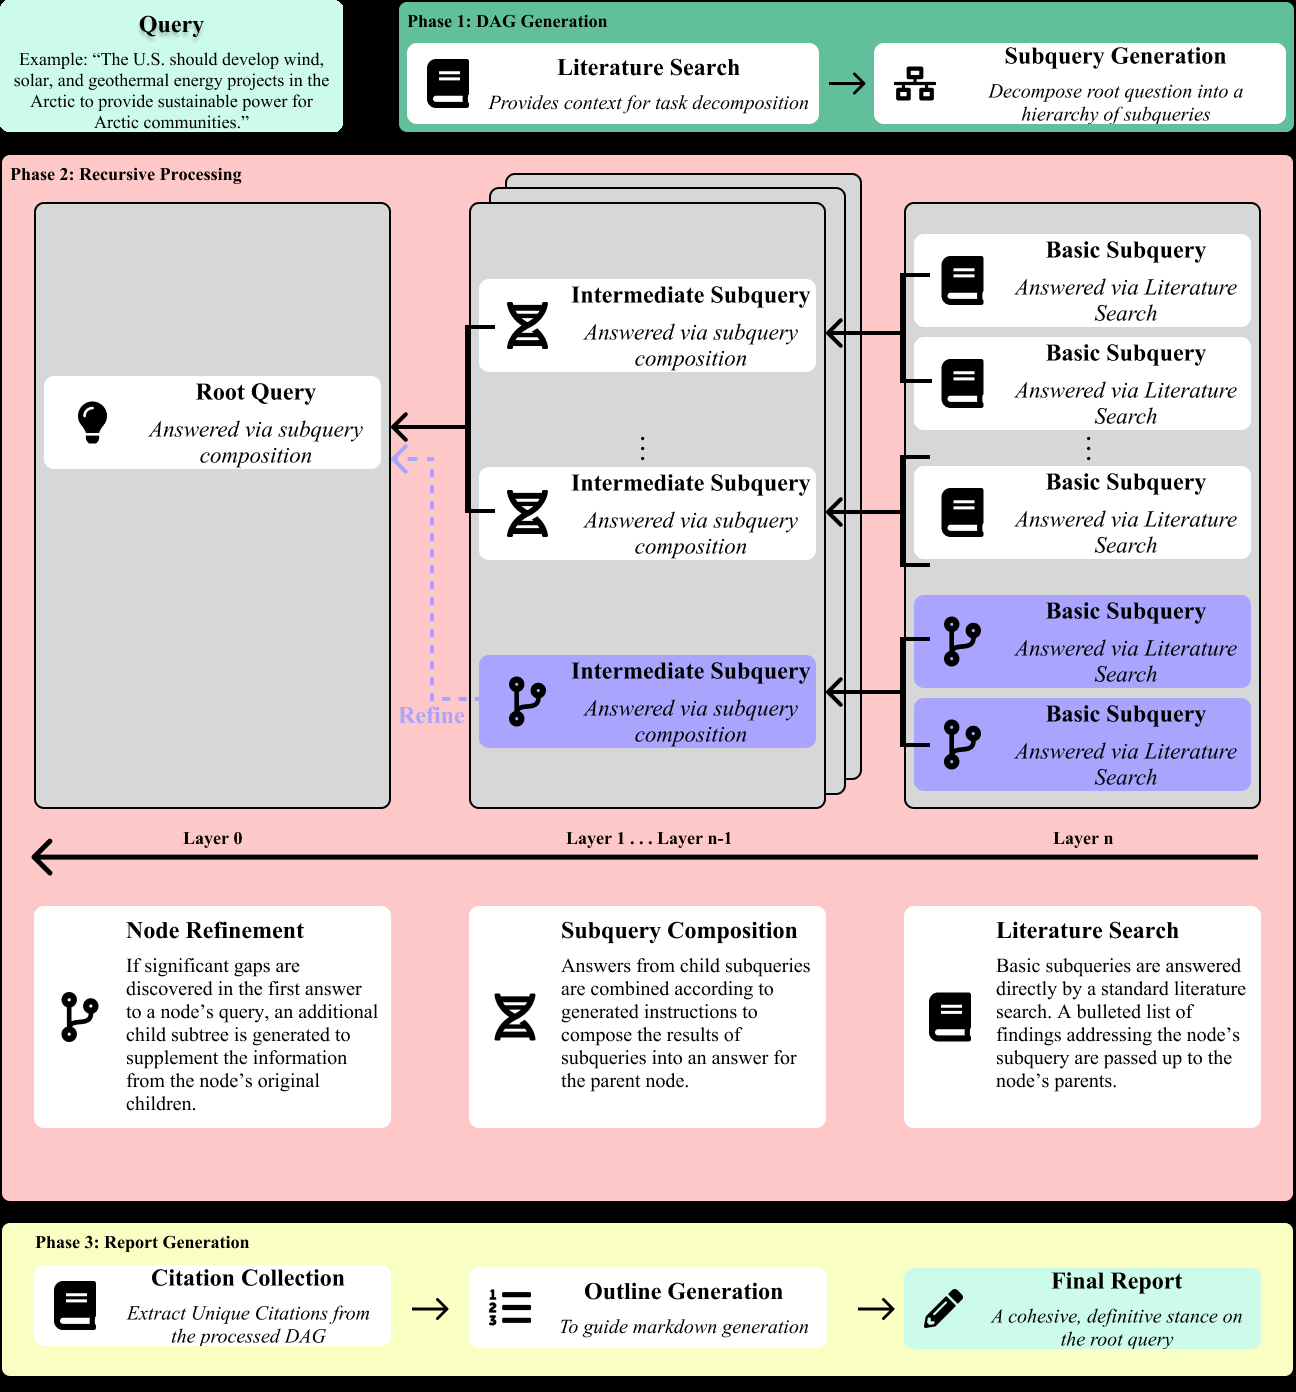
\includegraphics[width=\linewidth]{figs/pipeline.png}
\caption{The three phases of \sys{}. A literature search gives context for decomposing the query into a DAG of sub-queries (Phase 1). Leaves are answered by literature search, parents are composed from their children, and nodes with gaps are refined with new sub-trees (Phase 2). The answered DAG is turned into an outline and a report that argues the root answer (Phase 3).}
\label{fig:pipeline}
\end{figure}

\sys{} takes a research question and returns a report that argues an answer to it, with inline citations to web sources. It runs in three phases: DAG generation, recursive processing, and report generation. This section describes the pipeline as it was when the reports in \Cref{sec:experiments} were generated; \Cref{app:changes} describes the code versions involved and how the released code differs. Every language-model call is a DSPy signature \citep{khattab2024dspy}, reproduced in \Cref{app:prompts}.

\paragraph{Literature search.}
Both the planning phase and the leaf nodes use the same literature-search routine. A planning model turns a question into web queries, a retriever fetches results through the Serper API, scrapes the pages, embeds the passages with \texttt{text-embedding-3-large}, and keeps the passages closest to the query, and an answer model writes a cited answer from them. A completeness check decides whether to search again, up to a fixed number of retriever calls per question.

\paragraph{Phase 1: DAG generation.}
A short literature search on the root question gives the planner context. The planner then builds the DAG layer by layer. For each node in the current layer it generates child sub-questions, conditioned on the node's question, the literature summary, the children generated so far, and the structure of the whole DAG, so that siblings do not overlap and the children together answer the parent. The depth of the DAG, the total number of nodes, and the number of children per node are capped. A second pass writes composition instructions for every parent: given the parent's question and expected answer format and its children's questions, the model states how the children's answers combine into the parent's. The instructions reference children by their identifiers, so the dependency is explicit and can be checked later.

\paragraph{Phase 2: recursive processing.}
The DAG is sorted topologically and processed from the leaves to the root. Leaves are answered in parallel by literature search; the answer model writes bullet points in the node's expected format and keeps every citation from the search. Parents are composed in sequence: the children's answers, the composition instructions, and the expected format go to a synthesis model that may use only the children's content, must cite by the children's citation numbers, and must say so when children contradict each other. Citations are deduplicated as they pass up the graph.

A composed answer can still miss something the plan did not anticipate. After composing a parent, a gap explorer lists possible gaps in the answer, and a gap evaluator judges, at a configurable level of conservatism, whether any of them matters enough to act on. If so, the pipeline generates a sub-tree of new sub-questions for the gaps, attaches it under the parent, processes it like the rest of the DAG, and recomposes the parent. Each parent is refined at most once in the released configuration.

\paragraph{Phase 3: report generation.}
The answered DAG is serialized as text and its citations are collected into one numbered list. An outline model, instructed to argue a stance on the root question, writes an outline whose sections follow the hierarchy of the DAG. A report model then writes the report from the outline and the DAG, keeping the citations, taking the stance of the root answer, and titling the report with the claim rather than the question. Citation numbers are normalized and a bibliography is appended.

\begin{algorithm}[t]
\caption{\sys{}}
\label{alg:pipeline}
\begin{algorithmic}[1]
\Require motion $m$; limits on depth $d$, nodes $n$, children $c$; refinement rounds $\rho$
\State $L \gets \textsc{LiteratureSearch}(m)$ \Comment{context for planning}
\State $G \gets$ root $r$ with $q_r = m$
\For{each layer $\ell = 0, \dots, d-1$} \Comment{Phase 1}
  \For{each node $u$ at depth $\ell$}
    \State add children $\textsc{PlanChildren}(q_u, L, G, c)$ under $u$, within the node limit $n$
  \EndFor
\EndFor
\For{each parent $u$} $\kappa_u \gets \textsc{CompositionInstructions}(q_u, \{q_v : v \in C(u)\})$ \EndFor
\For{each node $u$ in topological order, leaves first} \Comment{Phase 2}
  \If{$u$ is a leaf}
    \State $(a_u, S_u) \gets \textsc{AnswerFromSearch}(q_u)$
  \Else
    \For{$k = 0, \dots, \rho$}
      \State $a_u \gets \textsc{Compose}(q_u, \{a_v\}_{v \in C(u)}, \kappa_u)$; \quad $S_u \gets \bigcup_{v \in C(u)} S_v$
      \State $\Delta \gets \textsc{FindGaps}(q_u, a_u)$
      \If{$k = \rho$ \textbf{or} $\Delta = \emptyset$} \textbf{break} \EndIf
      \State attach a sub-tree for $\Delta$ under $u$ and process it as in Phase 2
    \EndFor
  \EndIf
\EndFor
\State $O \gets \textsc{Outline}(m, a_r, G)$; \quad $R \gets \textsc{Report}(O, m, a_r, G)$ \Comment{Phase 3}
\State \Return $R$ with a bibliography of $\bigcup_v S_v$
\end{algorithmic}
\end{algorithm}

\paragraph{Cost.}
Let $|V_\text{leaf}|$ and $|V_\text{par}|$ be the numbers of leaves and parents after refinement. Each leaf costs one literature search, which is at least one query-generation call, one retrieval with embedding, one answer call, and one completeness check. Each parent costs one composition call per round and one gap check. Planning adds one call per parent for children and one for instructions, and writing adds two. The number of model calls is therefore about $4|V_\text{leaf}| + (3 + 2\rho)|V_\text{par}| + 3$, linear in the size of the graph, and leaves can be processed in parallel. The logged run in \Cref{app:dag} has \dagLeaves{} leaves and \dagParents{} parents, so it makes on the order of 40 model calls, compared with one or a few for a single-pass report.

\paragraph{Models and limits.}
The evaluation runs used GPT-4.1-mini for retrieval-side answer generation and planning, GPT-5 for DAG generation, synthesis, and report writing, and \texttt{text-embedding-3-large} for retrieval, all through Azure OpenAI; the released code also runs on the OpenAI API. The released defaults cap the DAG at depth 2, 50 nodes, and 10 children per node, with one retriever call per literature search and one refinement per parent.

\section{Experiments}
\label{sec:experiments}

Two evaluations compare \sys{} with OpenAI Deep Research \citep{openai2025deepresearch} and STORM \citep{shao2024storm}. The first is interactive: automated debates between \sys{} and Deep Research, scored by a language model. The second is a blind human scoring of full reports from all three systems. Both are small. Their size is stated here and discussed in \Cref{sec:discussion}.

\paragraph{Automated debates.}
Three motions were chosen to cover different kinds of reasoning: a moral one (moral systems rooted in theism are preferable to non-theistic systems), an economic and technical one (U.S.\ semiconductor manufacturers will outperform global peers over the next decade because of the CHIPS and Science Act), and a conceptual one (AI systems can be creative in the way humans are). Each motion was debated twice, with \sys{} and Deep Research exchanging the Pro and Con sides, for six transcripts. Each system researched the motion in its own way: \sys{} decomposed it into a DAG and composed its case from the answered nodes; Deep Research ran its default retrieval-and-synthesis pipeline. The debate itself was driven by GPT-5-mini, which produced alternating turns of 200--300 words for each side from that side's research and the opponent's previous turn.
% CHECK with Justin: confirm that the debate turns were generated by gpt-5-mini from each system's research output.
Transcripts were scored by GPT-4o-mini on stance consistency (fraction of turns that hold the assigned side), and on logical coherence, evidence integration, rebuttal specificity, persuasiveness, and fluency, each from 1 to 10, using the scoring framework of DeepResearch Bench, a course project by Abhinav Chinta and Charles Ding that is not published.

\paragraph{Human-coded reports.}
Ten motions were selected to need evidence synthesis and a stance rather than recall, spanning ethics, economics, policy, and technology; \Cref{tab:reports} lists them. Each system wrote one full report per motion. One author scored the thirty reports with the system identity hidden, on a rubric of supported-claims rate (the fraction of claims backed by a cited source), evidence utilization (the fraction of cited sources that the argument actually uses), logical connection quality (1--10), and whether the report holds a firm stance throughout. The rubric also had evidence relevance and originality; their recorded scores were identical across the three systems and could not be reconstructed, so they are omitted. There is one rater, so no agreement statistic exists, and the numbers below are means over ten reports without confidence intervals.

\paragraph{Released materials.}
The \sys{} and STORM reports for the ten motions are in the repository, with the prompts, the pipeline, and one complete logged run. The Deep Research reports and the debate transcripts were not retained. \Cref{sec:analysis,sec:citations} analyze the twenty retained reports and one logged run.
% CHECK with Jessie: are the Deep Research reports or the debate transcripts recoverable? If so, add them.

\section{Results}
\label{sec:results}

\begin{table}[t]
\centering
\small
\begin{tabular}{lccc}
\toprule
Metric & \sys{} & OpenAI Deep Research & Difference \\
\midrule
Stance consistency (\%) & \autoStanceDC & \autoStanceOAI & $+$23 \\
Logical coherence (1--10) & \autoCoherenceDC & \autoCoherenceOAI & $+$1.6 \\
Evidence integration (1--10) & \autoEvidenceDC & \autoEvidenceOAI & $+$1.8 \\
Rebuttal specificity (1--10) & \autoRebuttalDC & \autoRebuttalOAI & $+$1.7 \\
Persuasiveness (1--10) & \autoPersuasionDC & \autoPersuasionOAI & $+$0.9 \\
Fluency (1--10) & \autoFluencyDC & \autoFluencyOAI & $-$0.9 \\
\bottomrule
\end{tabular}
\caption{Automated debate scores, averaged over six transcripts (three motions, both sides), judged by GPT-4o-mini.}
\label{tab:auto}
\end{table}

\begin{table}[t]
\centering
\small
\begin{tabular}{lccc}
\toprule
Metric & \sys{} & OpenAI Deep Research & STORM \\
\midrule
Supported-claims rate & \humSupportedDC & \humSupportedOAI & \humSupportedStorm \\
Evidence utilization & \humUtilDC & \humUtilOAI & \humUtilStorm \\
Logical connection quality (1--10) & \humLogicDC & \humLogicOAI & \humLogicStorm \\
Firm stance (of 10 reports) & \humStanceDC & \humStanceOAI & \humStanceStorm \\
\bottomrule
\end{tabular}
\caption{Human-coded scores on ten reports per system, one blind rater, means over reports.}
\label{tab:human}
\end{table}

\paragraph{Automated debates.}
\Cref{tab:auto} gives the judge's scores. \sys{} scored higher on stance consistency, coherence, evidence integration, rebuttal specificity, and persuasiveness, and lower on fluency. The judge's notes point to the same cause in each motion. In the theism debate, \sys{}'s Pro case opened with the claim that moral objectivity needs a transcendent anchor and supported it with sub-claims that each carried evidence, such as volunteering rates in religious populations; Deep Research's Con case rested on the Euthyphro dilemma and repeated it across turns with little new evidence. With the sides reversed, \sys{} argued Con through meta-ethical consistency, cross-cultural variation in moral codes, and secular moral psychology, each with empirical or historical support, while Deep Research's Pro turns restated earlier points. In the semiconductor debate, \sys{} broke its Pro case into measurable claims (cost of capital under the subsidies, research-to-fab integration, supply-chain resilience, projected yields) and its Con case into quantified dependencies, including a projected plateau of U.S.\ fabrication share near 14\% by 2032; Deep Research's cases on both sides stayed qualitative. In the creativity debate, \sys{} split its reasoning into an empirical branch citing divergent-thinking benchmarks and a conceptual branch that defined creativity as novelty with usefulness; Deep Research argued from metaphysical objections without an operational definition. Across the six transcripts \sys{} made about twice as many evidence-linked claims per transcript. The fluency gap runs the other way: Deep Research's turns read more smoothly, and \sys{}'s denser citation of sub-claims costs some flow.

\paragraph{Human-coded reports.}
\Cref{tab:human} gives the rater's scores. \sys{} had the highest supported-claims rate (\humSupportedDC{} against \humSupportedOAI{} and \humSupportedStorm{}), used the largest share of its evidence (\humUtilDC{} against \humUtilOAI{} and \humUtilStorm{}), and had the highest logical connection score (\humLogicDC{} against \humLogicOAI{} and \humLogicStorm{}). It held a firm stance in \humStanceDC{} of ten reports; Deep Research did in \humStanceOAI{} and STORM in \humStanceStorm{}. The rater's notes describe the difference. On the moral-duty motion, \sys{} built a layered argument linking empathy to social trust, Deep Research gave a balanced account that did not decide, and STORM described positions without causal links between them. On the Federal Reserve motion, \sys{} argued through a chain from inflation control to wage stability, while Deep Research summarized both effects without connecting them. On the foundation-model investment motion, \sys{} produced a conditional argument (foundation models concentrate capital efficiency unless model saturation reduces marginal returns) that neither baseline matched. The supported-claims difference has a plausible source in the pipeline: every leaf answer is written from search results with citation markers, and every parent is composed only from its children, so a claim without a marker has little path into the report. Whether the markers point to the right sources is a separate question that the rubric did not ask, and \Cref{sec:citations} answers it. The firm-stance gap follows in part from the report prompt, which instructs the model to argue the root answer; \Cref{sec:discussion} returns to this.

\section{What the Reports Contain}
\label{sec:analysis}

The human scores in \Cref{tab:human} rest on one rater. The twenty retained reports, ten from \sys{} and ten from STORM on the same motions, allow a second look that needs no rater: measurements computed the same way on every report and compared motion by motion. Deep Research's reports were not retained, so this section compares \sys{} with STORM only. All differences are medians of the paired per-motion differences, with 95\% bootstrap intervals over motions \citep{efron1993bootstrap} and Wilcoxon signed-rank tests \citep{wilcoxon1945}; with ten pairs, the smallest attainable two-sided $p$ is 0.002. Bibliographies, headings, and markup are removed before counting.

\begin{table}[t]
\centering
\small
\resizebox{\linewidth}{!}{\begin{tabular}{lrrrrc}
\toprule
Measure & \sys{} & STORM & Difference & 95\% CI & Wins \\
\midrule
Citations per 100 words & 5.7 & 4.7 & $+$1.0 & [$+$0.0, $+$2.1] & 8/10 \\
Sentences with a citation & 0.46 & 0.60 & $-$0.15 & [$-$0.23, $-$0.09] & 0/10 \\
Distinct sources & 8 & 27 & $-$18 & [$-$24, $-$14] & 0/10 \\
Citations per source & 9.3 & 4.1 & $+$5.0 & [$+$1.7, $+$7.2] & 10/10 \\
Hedges per 1,000 words & 2.8 & 6.4 & $-$2.2 & [$-$7.3, $-$0.4] & 1/10 \\
Contrast markers per 1,000 words & 5.5 & 6.0 & $-$0.3 & [$-$0.8, $+$1.0] & 4/10 \\
Commitment markers per 1,000 words & 6.8 & 3.8 & $+$3.3 & [$+$0.4, $+$4.2] & 10/10 \\
Causal connectives per 1,000 words & 4.2 & 3.0 & $+$0.3 & [$-$0.5, $+$1.8] & 5/10 \\
Words & 1339 & 2426 & $-$1172 & [$-$1621, $-$617] & 0/10 \\
\bottomrule
\end{tabular}
}
\caption{Paired comparison of the ten \sys{} and ten STORM reports. Values are medians over motions; the difference is the median of the per-motion differences with a 95\% bootstrap interval; ``Wins'' counts motions where \sys{} is higher. Rates use the word lists in \Cref{app:lexicon}.}
\label{tab:text}
\end{table}

\begin{figure}[t]
\centering
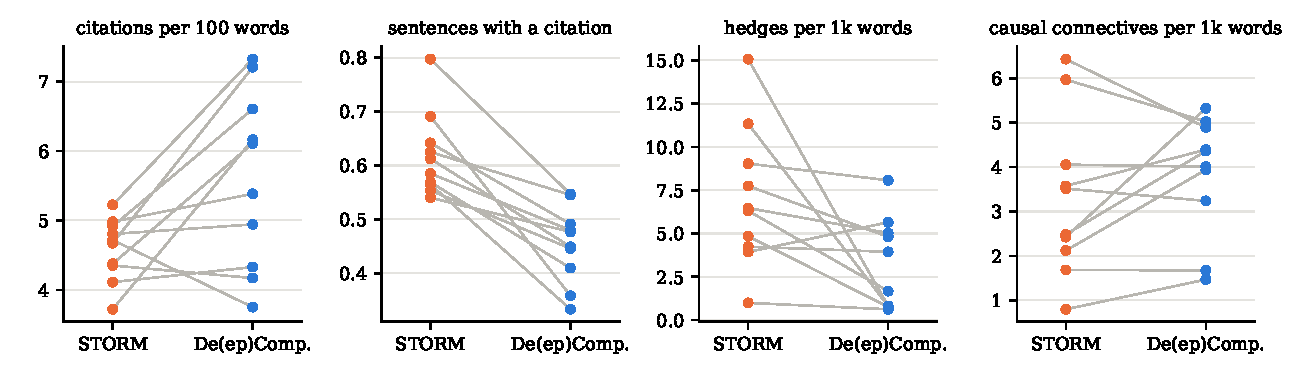
\includegraphics[width=\linewidth]{figs/paired_measures.pdf}
\caption{Four measures per motion. Each line joins the STORM report (left) and the \sys{} report (right) for one motion.}
\label{fig:paired}
\end{figure}

\paragraph{Stance.}
The lexical markers of stance agree with the rater. \sys{}'s reports use fewer hedges, words such as \emph{may}, \emph{could}, and \emph{suggests} that withhold commitment \citep{hyland2005metadiscourse}: \txHedgeDc{} per 1{,}000 words against \txHedgeSt{} for STORM, lower on nine of ten motions ($p = \txHedgeP$). They use more commitment markers such as \emph{must}, \emph{demonstrates}, and \emph{therefore}: \txCommitDc{} against \txCommitSt{} per 1{,}000 words, higher on all ten ($p = \txCommitP$). Contrast markers such as \emph{however} and \emph{on the other hand} occur at the same rate in both (\txContrastDc{} and \txContrastSt{}, $p = \txContrastP$), so \sys{} acknowledges the other side about as often as STORM does; it differs in committing after it does so.

The commitment is strongest at the top of the report and weaker at the end. \Cref{tab:stance} records, for each \sys{} report, which side of the motion it takes, whether its title is a claim, and how its final paragraph lands. \labTitleClaim{} of 10 titles state a claim, as the report prompt requires; all ten STORM reports open instead with a lead section that frames the question as a debate. The final paragraphs commit less: \labEndingFirm{} end firmly, \labEndingQualified{} qualify the title's claim (the creativity report concludes that human irreducibility persists ``but only provisionally''), \labEndingConditional{} make it conditional (the theism report concludes that the preference ``depends fundamentally on one's valuation'' of transcendent truth), and \labEndingCompromise{} replaces a yes-or-no answer with a compromise (the Federal Reserve report argues for ``balance''). One report takes the side opposite to the motion as worded, arguing that application-layer startups will outperform foundation-model developers. The stance instruction thus fixes the title and the executive summary, while the conclusion, written last from a DAG whose branches cover both sides, drifts toward the balanced synthesis the instruction was meant to prevent.

\paragraph{Connection.}
The rater scored \sys{} higher on logical connection, and the original write-up attributed this to causal chains between sub-claims. The rate of causal connectives (\emph{because}, \emph{leads to}, \emph{as a result}) does not show it: \txCausalDc{} per 1{,}000 words against \txCausalSt{}, higher on five of ten motions ($p = \txCausalP$). A connective count is a weak proxy for argument structure, so this does not contradict the rater, but it gives no independent support either.

\paragraph{Length and sourcing.}
\sys{}'s reports are shorter, \txWordsDc{} words of body text against \txWordsSt{}, on every motion. They cite more densely, \txCiteDensityDc{} citations per 100 words against \txCiteDensitySt{} ($p = \txCiteDensityP$), but from far fewer sources: a median of \txSourcesDc{} distinct sources in the body against \txSourcesSt{} for STORM, fewer on every motion, with each source cited \txCitesPerSourceDc{} times against \txCitesPerSourceSt{}. A smaller share of \sys{}'s sentences carry a citation at all (\txCitedShareDc{} against \txCitedShareSt{}, lower on every motion), because its dense citations cluster in bullet points while its connecting prose is uncited. The bibliographies tell the same story from the other side. Each \sys{} report lists a median of \bibMedDc{} retrieved sources (range \bibMinDc--\bibMaxDc) and separates them into ``cited'' and ``uncited''; the body cites \atUsedMin--\atUsedMax{} of them, a median of \atUsedShare\%. Most of what the pipeline retrieves never reaches the report.

\paragraph{Sources.}
\Cref{tab:sources} classifies the \srcN{} sources listed in \sys{}'s bibliographies by domain. Government sites make up \srcShareGovernment\%, academic publishers and university sites \srcShareAcademic\%, think tanks and other non-profit organizations \srcShareThinkTankOr\%, and company sites, blogs, and other pages the largest share, \srcShareCompanyBlogOrOther\%. News sites are almost absent. Of the \linkChecked{} links, \linkOkPct\% resolved when checked in October 2026, eleven months after the reports were written; \linkBlockedPct\% refused automated requests, and \linkDeadPct\% were gone or failing. The STORM exports carry citation numbers but no URLs, so the same check cannot be made for STORM.

\begin{table}[t]
\centering
\small
\begin{tabular}{lrr}
\toprule
Source type & Sources & Share \\
\midrule
Government & 45 & 13\% \\
Academic & 74 & 21\% \\
Think tank or NGO & 78 & 22\% \\
News or magazine & 3 & 1\% \\
Encyclopedia & 4 & 1\% \\
Company, blog, or other & 145 & 42\% \\
\bottomrule
\end{tabular}

\caption{Domains of the \srcN{} sources listed in \sys{}'s ten bibliographies, classified by host name.}
\label{tab:sources}
\end{table}

\paragraph{Structure.}
The two systems organize a report differently. STORM writes an encyclopedia article: a lead section that frames the question, a background section, and sections for the arguments on each side, often closing on the other side's case. \sys{} writes a brief: a claim as title, an executive summary that states the answer, sections that follow the branches of the DAG, and a conclusion. On the African Continental Free Trade Area, STORM opens by describing the agreement and its ratification history, while \sys{} opens by stating that the evidence ``overwhelmingly supports'' that the benefits outweigh the harms. On the moral-duty motion, STORM ends on critics who find equal obligation to strangers unrealistic, and \sys{} ends on a synthesis in which ``impartiality and partiality are not opposites,'' a softer position than its title.

\begin{table}[t]
\centering
\small
\begin{tabular}{p{5.2cm}lll}
\toprule
Motion & Side & Title & Final paragraph \\
\midrule
Human creativity will not remain fundamentally irreducible to\,\ldots & for & claim & qualified \\
Individuals have a moral duty to prioritize the well-being of\,\ldots & for & claim & qualified \\
Investing in companies developing foundation models -e.g., OpenAI,\,\ldots & against & claim & firm \\
Israel and Palestine should pursue a long-term joint economic zone\,\ldots & for & claim & firm \\
It is ethically justified for hedge funds to use alternative data\,\ldots & for & topic & conditional \\
Moral systems rooted in theism are preferable to non-theistic\,\ldots & for & claim & conditional \\
The benefits of the African Continental Free Trade Area outweigh\,\ldots & for & claim & firm \\
The U.S. Federal Reserve should prioritize maintaining high\,\ldots & neither & claim & compromise \\
The U.S. should develop wind, solar, and geothermal energy\,\ldots & for & claim & firm \\
U.S. semiconductor manufacturers will outperform global peers over\,\ldots & for & claim & firm \\
\bottomrule
\end{tabular}

\caption{Position of each \sys{} report. Side is relative to the motion as worded. The final paragraph is \emph{firm} if it restates the title's claim, \emph{qualified} if it limits the claim, \emph{conditional} if it makes the claim depend on unmet conditions or values, and \emph{compromise} if it answers neither side.}
\label{tab:stance}
\end{table}

\section{Citation Fidelity}
\label{sec:citations}

The rubric in \Cref{sec:experiments} counted a claim as supported when it carried a citation. It did not check whether the cited source says what the claim says. Attribution studies of generative search engines find that this check matters: in \citet{liu2023verifiability}, a quarter of citations did not support their sentence. This section measures it for \sys{}, finds that the evaluated reports fail it, traces the failure to two specific steps in the pipeline, and fixes them.

\subsection{A lexical attribution test}
For every sentence with bracketed citations, the test ranks all sources available to the document by TF-IDF cosine similarity \citep{salton1988termweighting} between the sentence and the source text, and records the rank of each cited source as a percentile (0 for the best match, 1 for the worst). If citations point to the sources a claim was written from, cited sources rank near the top. If citation numbers are scrambled, their percentile is uniform on $[0, 1]$, with median 0.5. Two summary statistics are reported: the median percentile of cited sources, and the share of claims whose single best-matching source is among those cited, against the share expected by chance. The test needs no model calls and runs on every report. It is lexical, so a source that paraphrases a claim in different words can rank low; the validation below measures how much this matters.

\paragraph{Validation.}
The leaf answers of the logged run (\Cref{app:dag}) are written by one model call directly from the retrieved excerpts they cite, so their citations are correct by construction. Against all \atValMeanCandidates{} sources of the run, the cited source is the best match for \atValBestCited{} of leaf claims, against \atValBestChance{} by chance, and the median percentile of cited sources is \atValMedianPct{} (95\% interval \atValPctLo--\atValPctHi). The evaluated reports cite full web pages rather than excerpts, so the test was repeated with the full text of the logged run's pages, fetched for this analysis: on the \atValPagesMeanCandidates{} pages that returned usable text, the cited page is the best match for \atValPagesBestCited{} of claims (chance \atValPagesBestChance). The test separates correct from scrambled citations clearly on both kinds of text.

\begin{table}[t]
\centering
\small
\resizebox{\linewidth}{!}{\begin{tabular}{lrrrrr}
\toprule
Setting & Claim--source pairs & Median rank percentile & Top-3 hit rate & Chance & Best match cited \\
\midrule
Leaf answers, own numbering & 63 & 0.04 [0.00, 0.08] & 0.83 & 0.12 & 0.96 (chance 0.10) \\
Leaf answers, own numbering, full pages & 24 & 0.00 [0.00, 0.11] & 0.88 & 0.30 & 0.84 (chance 0.13) \\
Leaf answers as a parent reads them, global numbering & 63 & 0.04 [0.00, 0.08] & 0.83 & 0.12 & 0.96 (chance 0.10) \\
Leaf answers as a parent read them, original pipeline & 63 & 0.12 [0.08, 0.16] & 0.49 & 0.12 & 0.52 (chance 0.10) \\
Final report, logged run & 173 & 0.48 [0.44, 0.52] & 0.06 & 0.12 & 0.04 (chance 0.10) \\
Evaluated reports, all listed sources & 491 & 0.47 [0.40, 0.53] & 0.18 & 0.14 & 0.14 (chance 0.10) \\
Evaluated reports, cited sources only & 491 & 0.43 [0.40, 0.50] & 0.56 & 0.51 & 0.41 (chance 0.36) \\
\bottomrule
\end{tabular}
}
\caption{Attribution of cited claims. Each row ranks every available source by lexical similarity to each cited claim. The median rank percentile of the cited sources is 0 if they are always the best match and 0.5 if citations are random (95\% bootstrap interval in brackets). The top-3 hit rate is the share of cited sources ranked in the top three; chance is its expected value under random citation. The last column is the share of claims whose best match is cited.}
\label{tab:attribution}
\end{table}

\begin{figure}[t]
\centering
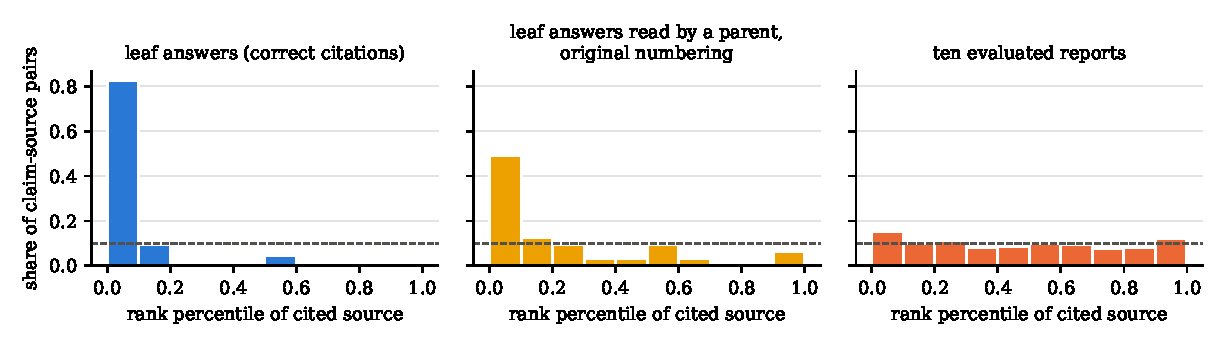
\includegraphics[width=\linewidth]{figs/attribution.pdf}
\caption{Rank percentile of each cited source among all available sources. Correct citations pile up at 0 (left). The evaluated reports are flat, as random citations would be (right). The middle panel shows the leaf answers as a parent node in the repository version read them (\Cref{sec:mechanism}). The dashed line marks the uniform distribution.}
\label{fig:attribution}
\end{figure}

\subsection{Results}
\Cref{tab:attribution} and \Cref{fig:attribution} give the results. In the ten evaluated reports, the \atEvalClaims{} cited claims carry \atEvalPairs{} claim--source pairs. The median percentile of the cited sources among all listed sources is \atEvalMedianPct{} (\atEvalPctLo--\atEvalPctHi), indistinguishable from 0.5, and the claim's best match is cited for \atEvalBestCited{} of claims against \atEvalBestChance{} by chance. Restricting the candidates to the sources the report actually cites, a median of \atEvalCitedMeanCandidates{} per report, the best match is cited for \atEvalCitedBestCited{} of claims against \atEvalCitedBestChance{} by chance. The final report of the logged run, produced with the same report-writing step, is also at chance (median percentile \atLogMedianPct). By this test, the citations in the evaluated reports carry almost no information about which source supports which claim.

Two cases from the theism report show what this looks like. A bullet stating that ``non-theistic systems such as Confucianism, Buddhism, and Stoicism achieved moral stability'' without divine law cites five sources, all of them arguments for the existence of God from the moral law. A bullet on ancient Egyptian, Israelite, and Vedic societies cites ``A Beginner's Guide to the Moral Argument.'' The claims may well be true; the cited sources are not where they came from.

\subsection{Mechanism}
\label{sec:mechanism}
The code that produced the evaluated reports is not public (\Cref{app:changes}), but the repository version from a week earlier is, together with a run it produced, and it loses provenance at two steps. Both are consistent with the symptoms of the evaluated reports, though they cannot be confirmed in that version's code.

\paragraph{Local numbers read in a merged list.}
A leaf answer cites its own sources as [1] to [$k$]. When a parent is composed, the repository version merges its children's sources into one deduplicated list numbered [1] to [$m$] and gives the synthesis model this list with the instruction to cite by its numbers, but it passes the children's answers with their original leaf-local numbers. A ``[1]'' copied from the second child therefore points to the first child's first source. The middle rows of \Cref{tab:attribution} replay this on the logged run. Read in the parent's merged list, the leaf claims' citations still hit the best match for \atOldBestCited{} of claims, the correct ones from each parent's first child, but no longer the \atValBestCited{} they had in their own numbering. Every level of the DAG applies this scrambling again.

\paragraph{Node identifiers instead of sources.}
The composition instructions generated in Phase 1 tell the synthesis model to credit children by node identifier so that dependencies can be traced, while the synthesis prompt tells it to cite sources by number. In the logged run, \dagParents{} nodes were composed, counting the root. Three of them, the root among them, followed the composition instructions and wrote references such as ``(node\_3)'' after their claims, with no source numbers at all; one cited by number. The report writer then receives a root answer without source citations and an instruction to cite by number, and assigns numbers it has no basis for, which is why the logged report is at chance.

\subsection{Fix}
The released code makes provenance explicit. Every source receives one global number when any node first retrieves it, and leaf answers are rewritten from local to global numbers before they are stored, so children and parent share one numbering and the report's bibliography uses it too. After composition, node identifiers in the parent's answer are replaced by the global citations of those children, and numbers outside the parent's sources are removed. The synthesis prompt and the composition-instruction prompt both now say to cite sources by number and never by node. The lexical test above is included as an audit that can flag claims whose cited sources rank in the bottom half. Replayed on the logged run, the leaf claims keep their attribution under the new numbering (\atFixBestCited{} best-match rate, the same as the leaves themselves). Whether the report writer then preserves it end to end requires new runs, which are not part of this study; the test makes that check cheap.

\subsection{Implications}
The supported-claims rate in \Cref{tab:human} counted citation markers, so it measures how consistently \sys{} attaches citations, which it does more densely than STORM (\Cref{sec:analysis}), not whether its claims are supported by what they cite. The evaluated reports should not be read as better grounded than the baselines; the evaluation does not show that. The same test applies to any system with inline citations; STORM's exports lacked URLs and Deep Research's reports were not retained, so neither baseline could be checked here.

\section{Discussion}
\label{sec:discussion}

\paragraph{What the results support.}
Three findings hold up across methods. \sys{} writes decisive reports: the rater found a firm stance far more often than in either baseline, and the lexical measurements agree, with fewer hedges on nine of ten motions and more commitment markers on all ten. It writes compact, densely cited reports organized around a claim. And its recursive composition, as implemented, does not preserve which source supports which claim, so its citations should not be trusted until the fix in \Cref{sec:citations} is validated end to end. The rater's higher scores for supported claims and evidence use reflect the first two findings, citations attached consistently in a compact report, more than the third.

\paragraph{The stance result is partly a prompt.}
The report prompt tells the model to argue the root answer and not to hedge, so a high firm-stance rate was expected from the prompt alone. The decomposition contributes a root answer with a definite format for the prompt to argue, but the experiment does not separate the two. The analysis adds a complication: titles and summaries commit, while half of the conclusions qualify or condition the claim. The final writing step sees a DAG whose branches cover both sides, and the balanced material reasserts itself at the end. An ablation that keeps the DAG and removes the stance instruction, one that keeps the instruction and removes the DAG, and one that asks for a conclusion consistent with the title would separate these effects.

\paragraph{Why provenance fails in recursive composition.}
Citations are pointers into a list, and the pipeline rebuilt the list at each level while copying the pointers unchanged. Any system that composes cited text recursively, by summarizing summaries or merging the outputs of sub-agents, faces the same risk, and the error is invisible to a reader and to a rubric that counts citation markers. Two design rules avoid it: give every source one identifier for the whole run, and never let a model refer to intermediate results by an identifier that the final text cannot resolve to a source. A lexical audit like the one here is a cheap check that either rule was followed, and attribution metrics with entailment models \citep{rashkin2023ais, gao2023alce} are a stronger one.

\paragraph{Scale and raters.}
Ten motions and six transcripts are too few for precise estimates, and the human scores come from one rater who is an author, blind to the system but not to the study. The judge in the debates is a small model applying a rubric from an unpublished course project. Two rubric metrics were dropped because their records were unusable. The paired measurements in \Cref{sec:analysis} have no rater, but they are lexical proxies, and the stance labels in \Cref{tab:stance} come from one reading.

\paragraph{Uncontrolled factors.}
The three systems differ in model, search backend, and prompt, so the comparison measures systems, not the decomposition alone. STORM was built to write balanced encyclopedia articles and is scored here on a task it was not designed for; its low firm-stance count is its design, not a failure. Deep Research's reports were produced in a commercial product whose internals and model version are not controllable. A controlled study would hold the backbone model and the search API fixed across a flat search agent, STORM, and \sys{}, run the ablations above, and score attribution with the test in \Cref{sec:citations} alongside human judgments.

\paragraph{Cost.}
A \sys{} run makes on the order of four model calls per leaf and a few per parent (\Cref{sec:method}), so its cost grows linearly with the graph, at several times the calls of a single-pass report. Most of what it retrieves is never cited: a median of \atUsedShare\% of the listed sources reach the report body. Pruning sources that no claim uses before the final step would shorten the bibliography without changing the argument.

\section{Conclusion}
\label{sec:conclusion}
\sys{} turns a motion into a DAG of sub-questions, answers it from the leaves up under generated composition instructions, extends the graph where answers are incomplete, and writes a report that argues the result. On ten debate motions and six automated debates it produced more decisive and more densely cited arguments than OpenAI Deep Research and STORM, at some cost in fluency and with conclusions that soften more often than its titles. Its citations, however, did not point to the sources their claims came from: recursive composition lost provenance at two identifiable steps. The released code fixes both and includes a validated attribution test that needs no model calls. The next step is to rerun the comparison with a fixed backbone and search API, the stance ablations, more motions and raters, and attribution measured on every system.


\bibliography{refs}
\bibliographystyle{colm2026_conference}

\clearpage
\appendix
\section{Prompts}
\label{app:prompts}
The instructions of the DSPy signatures used for the evaluation runs, verbatim. Input and output fields are omitted.

\begin{lstlisting}[title={LayerChildGenerationSignature (Phase 1, one layer of children)}]
Generate children for a specific parent node in the research DAG.
You are a research planning expert. Given a parent research question and the current DAG structure, generate focused sub-questions that can be answered independently to collectively answer the parent question. Look at the entire DAG context to ensure coherence and avoid duplication.
Guidelines:
1. Generate focused, standalone sub-questions that collectively answer the parent
2. Consider the existing DAG structure to maintain coherence
3. Respect the max_children limit strictly
4. Each child should be answerable independently
5. Output format should always be "list" (bullet points)
\end{lstlisting}

\begin{lstlisting}[title={CompositionInstructionSignature (Phase 1, per parent)}]
Write explicit parent composition instructions referencing each child node.
Given a parent node and its children, explain exactly how the child answers will be combined to produce the parent's output. Always reference children by their IDs so downstream steps can trace dependencies unambiguously.
\end{lstlisting}

\begin{lstlisting}[title={LeafNodeResearcher (Phase 2, leaves)}]
Answer a leaf node research task using literature search results.
Given literature search results and the expected output format, provide an answer that strictly adheres to the format requirements.
Format types and requirements:
- boolean: Provide "Yes." or "No." followed by a single sentence justification with citations.
- short_answer/list/report: Provide 3-5 bullet points ('- ' prefix) summarizing key takeaways with citations.
- table_csv/json: Provide structured data (CSV or JSON) with inline citations in headers or cells.
CRITICAL: Preserve all citations from the literature search in [X] format. Do not add citations that aren't in the source material.
\end{lstlisting}

\begin{lstlisting}[title={ParentNodeSynthesizer (Phase 2, parents)}]
Synthesize answers from child nodes to answer a parent node's research task.
Given the answers from all child subtasks and composition instructions, combine them to produce the answer for the parent task in the required format.
CRITICAL RULES:
1. Use ONLY the information from the child results - no external knowledge
2. Follow the composition instructions exactly
3. When citing evidence, use the citation numbers [1], [2], etc. from the AVAILABLE CITATIONS section - do NOT reference child nodes by name
4. Output in the specified format
5. If child results contradict, acknowledge and explain the contradiction
\end{lstlisting}

\begin{lstlisting}[title={GapExplorer (Phase 2, refinement, first pass)}]
Explore potential gaps that could enhance the composed answer.
This is the FIRST PASS - be creative and identify any areas where the answer could be improved, even if they're minor enhancements. Don't filter yet.
Think about: missing perspectives or viewpoints; unaddressed sub-questions or aspects; areas that could use more depth or detail; counterarguments or alternative viewpoints not covered; quantitative data or evidence gaps; temporal or geographic coverage gaps; edge cases or exceptions not mentioned.
Return a list of potential gaps, even if they seem minor. The second pass will determine which ones are critical enough to warrant refinement.
\end{lstlisting}

\begin{lstlisting}[title={GapImportanceEvaluator (Phase 2, refinement, second pass)}]
Evaluate whether identified gaps are important enough to warrant refinement.
This is the SECOND PASS - evaluate gaps based on the specified conservatism level.
CONSERVATISM MODES:
- "conservative": Only flag gaps that are CRITICAL - the answer would be misleading or fundamentally incomplete without this information. Default to NOT refining.
- "balanced": Flag gaps that would SIGNIFICANTLY improve the answer's completeness, depth, or accuracy. Be moderate - refine if the gap meaningfully enhances quality.
- "aggressive": Flag gaps that would improve the answer, even if moderately. Refine if the gap would add value, even if not critical.
Consider: Would adding this information fundamentally change the answer's conclusion? Is this gap misleading or would it cause the answer to be wrong? Would a reasonable reader say the answer is incomplete without this? Is this a core aspect of the question that's missing? How much would this gap improve the answer's quality?
Provide a confidence score (0.0-1.0) indicating how confident you are that refinement is warranted.
\end{lstlisting}

\begin{lstlisting}[title={OutlineFromDAGSignature (Phase 3)}]
Generate a report outline that structures a persuasive argument from DAG research.
The DAG represents a research question decomposed into sub-questions. Each node answered a question through research. The root node has the final answer; child nodes contain supporting evidence that led to that answer.
Create an outline for a persuasive report arguing a definitive stance for the root answer. Use the DAG's hierarchy to organize evidence: child findings support parent conclusions. Structure as a logical argument (Executive Summary, Evidence Sections, Conclusion).
REQUIREMENTS: Start with Executive Summary stating root answer prominently; organize body sections to build argument logically using DAG hierarchy; use ## for main sections, ### for subsections; design for prose writing (paragraphs, not just lists); base outline ONLY on content actually present in root_answer (no placeholders).
\end{lstlisting}

\begin{lstlisting}[title={ReportFromDAGSignature (Phase 3)}]
Generate a comprehensive final report from the DAG results.
The report must: 1. Start with the root answer prominently (matching its format) 2. Follow the provided outline structure 3. Incorporate findings from all DAG nodes 4. Take a clear stance that matches the root answer 5. Preserve all citations [X] from the DAG 6. Be well-written, coherent, and comprehensive
CRITICAL STANCE ALIGNMENT: If root answer is "Yes" (boolean), the report must argue FOR that position. If root answer is "No" (boolean), the report must argue AGAINST. If root answer is a list, the report should be organized around those items. The report's conclusion must align with the root answer. Do not contradict or hedge against the root answer's stance.
FORMATTING REQUIREMENTS: The report title (# heading) should be the CLAIM, not the question. Use proper markdown; write in prose paragraphs with supporting bullet points where appropriate; do not include internal node references in the output; only use citation numbers like [1], [2], [3]; every section must contain substantive content from the dag_results; do not include a bibliography section (it is added later).
\end{lstlisting}

\section{An Example DAG}
\label{app:dag}
\Cref{fig:dag} shows the DAG from a logged run on the motion ``Should the United States federal government substantially increase social services for persons living in poverty?'' with depth capped at 2. The planner split the root into the current landscape of services and the likely effects of expanding them, and each of those into two leaves. After composing the landscape node, the refinement check judged that child care and family tax credits were missing, and the pipeline attached a refinement sub-tree with two new leaves (shaded). The run's \dagLeaves{} leaves retrieved \dagLeafSources{} distinct sources, \dagLeafSourcesMean{} per leaf, and \dagRootFromRefinement{} of the root's \dagRootSources{} sources came from the refinement sub-tree, so refinement added about a third of the evidence. The final report has \dagReportWords{} words and \dagReportCitations{} citations and cites all \dagReportSources{} sources; \Cref{sec:citations} shows that its citations nonetheless do not match their claims. The full log, with every node's answer and citations, is in the repository.

\begin{figure}[t]
\centering
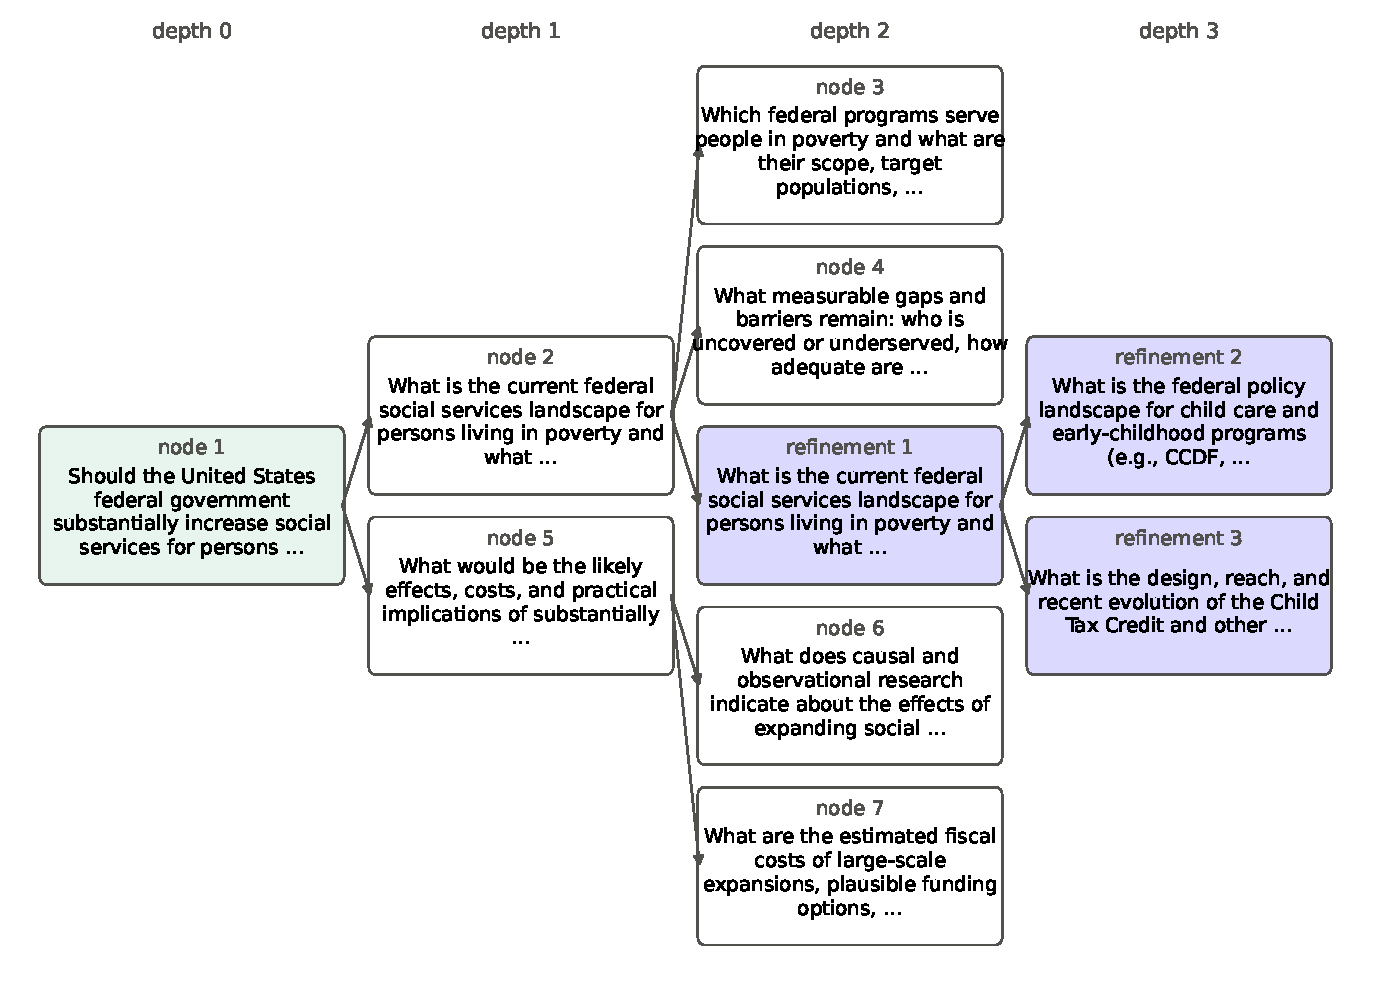
\includegraphics[width=\linewidth]{figs/example_dag.pdf}
\caption{A generated and refined DAG. Arrows point from parent to child. Shaded nodes were added by refinement after the composed answer of node 2 was judged incomplete.}
\label{fig:dag}
\end{figure}

\section{Code Versions}
\label{app:changes}
Three versions of the pipeline are involved, and only two are available.
\begin{enumerate}
    \item \textbf{Evaluated version.} The reports in \Cref{sec:experiments,sec:analysis} were finalized on 2 December 2025. Its prompts are the ones in \Cref{app:prompts}, taken from the authors' course write-up: the DAG is generated one layer at a time, composition instructions are written in a second pass, gaps are found by a two-pass explorer and evaluator, and the bibliography separates cited from uncited sources. This version's code is not in the public repository.
    \item \textbf{Repository version.} The last commit in the repository, from 26 November 2025, generates the whole DAG and its composition instructions in one call (\texttt{FullDAGGenerationSignature}) and checks gaps with one validator (\texttt{CompositionValidator}) that returns none unless a core aspect is missing. The logged run in \Cref{app:dag} comes from this version. Its citation handling is the one analyzed in \Cref{sec:mechanism}. The course write-up reports that citations were later given global numbers; that change is not in this version.
    \item \textbf{Released version.} The repository version with the provider made configurable, legacy code removed, and the citation fix of \Cref{sec:citations}: global citation numbers, node-reference expansion, the updated prompts, and the attribution audit (\texttt{utils/citations.py}, \texttt{utils/attribution\_audit.py}), with tests that replay the logged run.
\end{enumerate}
% CHECK with Justin: is the evaluated version (Gradescope submission) available? If so, add it to the repository and confirm whether its parent composition still passed leaf-local citation numbers.

\section{Report Statistics by Motion}
\label{app:reports}
\Cref{tab:reports} gives the length and sourcing of each retained report. The medians in \Cref{tab:text} are computed from these values.

\begin{table}[t]
\centering
\small
\begin{tabular}{p{6.4cm}rrrrr}
\toprule
Motion & \multicolumn{3}{c}{\sys{}} & \multicolumn{2}{c}{STORM} \\
\cmidrule(lr){2-4}\cmidrule(lr){5-6}
 & words & cited & listed & words & cited \\
\midrule
Human creativity will not remain fundamentally irreducible to artificial intelligence when\,\ldots & 1{,}235 & 8 & 31 & 1{,}991 & 32 \\
Individuals have a moral duty to prioritize the well-being of strangers equally to the\,\ldots & 1{,}523 & 8 & 38 & 1{,}887 & 22 \\
Investing in companies developing foundation models -e.g., OpenAI, Anthropic- will yield\,\ldots & 1{,}247 & 9 & 37 & 2{,}712 & 30 \\
Israel and Palestine should pursue a long-term joint economic zone to promote regional\,\ldots & 1{,}363 & 9 & 35 & 3{,}763 & 35 \\
It is ethically justified for hedge funds to use alternative data sources (e.g., satellite\,\ldots & 1{,}594 & 10 & 30 & 2{,}797 & 24 \\
Moral systems rooted in theism are preferable to non-theistic moral systems. & 1{,}393 & 11 & 36 & 2{,}010 & 23 \\
The benefits of the African Continental Free Trade Area outweigh the harms & 1{,}195 & 7 & 38 & 2{,}376 & 32 \\
The U.S. Federal Reserve should prioritize maintaining high interest rates over stimulating\,\ldots & 1{,}226 & 7 & 32 & 3{,}265 & 24 \\
The U.S. should develop wind, solar, and geothermal energy projects in the Arctic to\,\ldots & 1{,}315 & 13 & 33 & 2{,}477 & 32 \\
U.S. semiconductor manufacturers will outperform global peers over the next decade due to\,\ldots & 1{,}605 & 8 & 39 & 2{,}014 & 23 \\
\bottomrule
\end{tabular}

\caption{Body length in words and number of distinct sources cited in the body of each retained report, and, for \sys{}, the number of sources listed in its bibliography.}
\label{tab:reports}
\end{table}

\section{Stance Labels}
\label{app:stance}
The labels in \Cref{tab:stance} come from reading each \sys{} report's title and final paragraph. The repository records each label with a short quotation from the final paragraph (\texttt{data/reports/stance\_labels.json}) so that it can be checked.
% CHECK with Jessie and Justin: read the ten final paragraphs and confirm the labels.

\section{Word Lists}
\label{app:lexicon}
Rates in \Cref{tab:text} count whole-word, case-insensitive matches per 1{,}000 words of body text. The lists follow the categories of \citet{hyland2005metadiscourse}, adapted to argumentative reports.
\begin{description}
\item[Hedges.] may, might, could, possibly, perhaps, arguably, potentially, appears, appear, seems, seem, suggests, suggest, likely, unlikely, uncertain, unclear, debated, contested, controversial, depends, depending, can be, to some extent, in some cases, remains open.
\item[Contrast markers.] however, on the other hand, conversely, while, whereas, although, though, nevertheless, nonetheless, critics, opponents, proponents, detractors, both sides.
\item[Commitment markers.] must, should, clearly, demonstrates, demonstrate, shows, show, proves, establishes, therefore, thus, decisively, undeniably, strongly, essential, necessary, outweigh, outweighs, superior, preferable.
\item[Causal connectives.] because, therefore, thus, hence, as a result, consequently, leads to, lead to, led to, results in, result in, resulting in, drives, drive, causes, cause, due to, which means, so that, enables, enable, reduces, increases, raises, lowers.
\end{description}


\end{document}
